\documentclass[sigchi-a, authorversion]{acmart}
\usepackage{booktabs} % For formal tables
\usepackage{ccicons}  % For Creative Commons citation icons

% Copyright
%\setcopyright{none}
\setcopyright{acmcopyright}
%\setcopyright{acmlicensed}
%\setcopyright{rightsretained}
%\setcopyright{usgov}
%\setcopyright{usgovmixed}
%\setcopyright{cagov}
%\setcopyright{cagovmixed}


% DOI
\acmDOI{10.475/123_4}

% ISBN
\acmISBN{123-4567-24-567/08/06}

%Conference
\acmConference[WOODSTOCK'97]{ACM Woodstock conference}{July 1997}{El
  Paso, Texas USA} 
\acmYear{1997}
\copyrightyear{2016}

\acmPrice{15.00}

%\acmBadgeL[http://ctuning.org/ae/ppopp2016.html]{ae-logo}
\acmBadgeR[http://ctuning.org/ae/ppopp2016.html]{ae-logo}

\begin{document}
\title{SIGCHI Extended Abstracts Sample File}

\author{First Author}
\affiliation{%
  \institution{University of Author}
  \city{Authortown}
  \state{CA} 
  \postcode{94022} 
  \country{USA} }
\email{author1@anotherco.edu}

\author{Second Author}
\affiliation{%
  \position{VP, Authoring}
  \institution{Authorship Holdings, Ltd.}
  \city{Awdur} 
  \postcode{SA22 8PP}
  \country{UK}}
\email{author2@author.ac.uk}

\author{Third Author \\
  Fourth Author}
\affiliation{%
  \institution{L\={e}khaka Labs}
  \city{Bengaluru} \postcode{560 080} \country{India}}
\email{author3@another.com} 
\email{author4@another.com}

\author{Fifth Author}
\affiliation{\institution{YetAuthorCo, Inc.}
  \city{Authortown} \state{BC}
  \postcode{V6M 22P} \country{Canada}}
\email{author5@anotherco.com} 

\author{Sixth Author}
\affiliation{\institution{Universit\'e de Auteur-Sud}
  \city{Auteur} \postcode{40222} \country{France}}
\email{author6@author.fr} 

\author{Seventh Author}
\affiliation{\institution{University of Umbhali}
  \city{Pretoria} \country{South Africa}}
\email{author7@umbhaliu.ac.za} 

% The default list of authors is too long for headers}
\renewcommand{\shortauthors}{F. Author et al.}


%
% The code below should be generated by the tool at
% http://dl.acm.org/ccs.cfm
% Please copy and paste the code instead of the example below. 
%
\begin{CCSXML}
<ccs2012>
 <concept>
  <concept_id>10010520.10010553.10010562</concept_id>
  <concept_desc>Computer systems organization~Embedded systems</concept_desc>
  <concept_significance>500</concept_significance>
 </concept>
 <concept>
  <concept_id>10010520.10010575.10010755</concept_id>
  <concept_desc>Computer systems organization~Redundancy</concept_desc>
  <concept_significance>300</concept_significance>
 </concept>
 <concept>
  <concept_id>10010520.10010553.10010554</concept_id>
  <concept_desc>Computer systems organization~Robotics</concept_desc>
  <concept_significance>100</concept_significance>
 </concept>
 <concept>
  <concept_id>10003033.10003083.10003095</concept_id>
  <concept_desc>Networks~Network reliability</concept_desc>
  <concept_significance>100</concept_significance>
 </concept>
</ccs2012>  
\end{CCSXML}

\ccsdesc[500]{Computer systems organization~Embedded systems}
\ccsdesc[300]{Computer systems organization~Redundancy}
\ccsdesc{Computer systems organization~Robotics}
\ccsdesc[100]{Networks~Network reliability}

% We no longer use \terms command
%\terms{Theory}

\begin{abstract}
  UPDATED---\today. This sample paper describes the formatting
  requirements for SIGCHI Extended Abstract Format, and this sample
  file offers recommendations on writing for the worldwide SIGCHI
  readership. Please review this document even if you have submitted
  to SIGCHI conferences before, as some format details have changed
  relative to previous years. Abstracts should be about 150
  words. Required.
\end{abstract}


\keywords{Authors' choice; of terms; separated; by
  semicolons; include commas, within terms only; required.}



\maketitle

\begin{sidebar}
  \textbf{Good Utilization of the Side Bar} 
  
  \textbf{Preparation:} Do not change the margin
  dimensions and do not flow the margin text to the
  next page. 
  
  \textbf{Materials:} The margin box must not intrude
  or overflow into the header or the footer, or the gutter space
  between the margin paragraph and the main left column. 
  
  \textbf{Images \& Figures:} Practically anything
  can be put in the margin if it fits. Use the
  \texttt{{\textbackslash}marginparwidth} constant to set the
  width of the figure, table, minipage, or whatever you are trying
  to fit in this skinny space.

  \caption{This is the optional caption}
  \label{bar:sidebar}
\end{sidebar}

\begin{figure}
  
\includegraphics[width=\marginparwidth]{sigchi-logo}
  \caption{Insert a caption below each figure.}
  \label{fig:sample}
\end{figure}


\section{Introduction}
This format is to be used for submissions that are published in the
conference publications. We wish to give this volume a consistent,
high-quality appearance. We therefore ask that authors follow some
simple guidelines. In essence, you should format your paper exactly
like this document. The easiest way to do this is to replace the
content with your own material.


\section{ACM Copyrights \& Permission}
Accepted extended abstracts and papers will be distributed in the
Conference Publications. They will also be placed in the ACM Digital
Library, where they will remain accessible to thousands of researchers
and practitioners worldwide. To view the ACM's copyright and
permissions policy, see:
\url{http://www.acm.org/publications/policies/copyright_policy}.


\section{Page Size}
All SIGCHI submissions should be US letter (8.5 $\times$ 11
inches). US Letter is the standard option used by this \LaTeX\
template.

\section{Text Formatting}
Please use an 8.5-point Verdana font, or other sans serifs font as
close as possible in appearance to Verdana in which these guidelines
have been set. Arial 9-point font is a reasonable substitute for
Verdana as it has a similar x-height. Please use serif or
non-proportional fonts only for special purposes, such as
distinguishing \texttt{source code} text.

\subsubsection{Text styles}
The \LaTeX\ template facilitates text formatting for normal (for body
text); heading 1, heading 2, heading 3; bullet list; numbered list;
caption; annotation (for notes in the narrow left margin); and
references (for bibliographic entries). Additionally, here is an
example of footnoted\footnote{Use footnotes sparingly, if at all.}
text. As stated in the footnote, footnotes should rarely be used.

\begin{table}
  \caption{Table captions should be placed above the table. We
    recommend table lines be 1 point, 25\% black. Minimize use of
    table grid lines.}
  \label{tab:table1}
  \begin{tabular}{l r r r}
%     \toprule
    & & \multicolumn{2}{c}{\small{\textbf{Test Conditions}}} \\
    \cmidrule(r){3-4}
    {\small\textit{Name}}
    & {\small \textit{First}}
      & {\small \textit{Second}}
    & {\small \textit{Final}} \\
    \midrule
    Marsden & 223.0 & 44 & 432,321 \\
    Nass & 22.2 & 16 & 234,333 \\
    Borriello & 22.9 & 11 & 93,123 \\
    Karat & 34.9 & 2200 & 103,322 \\
     \bottomrule
  \end{tabular}
\end{table}


\subsection{Language, style, and content}
The written and spoken language of SIGCHI is English. Spelling and
punctuation may use any dialect of English (e.g., British, Canadian,
US, etc.) provided this is done consistently. Hyphenation is
optional. To ensure suitability for an international audience, please
pay attention to the following:
\begin{itemize}
\item Write in a straightforward style. Use simple sentence
  structure. Try to avoid long sentences and complex sentence
  structures. Use semicolons carefully.
\item Use common and basic vocabulary (e.g., use the word ``unusual''
  rather than the word ``arcane'').
\item Briefly define or explain all technical terms. The terminology
  common to your practice/discipline may be different in other design
  practices/disciplines.
\item Spell out all acronyms the first time they are used in your
  text. For example, ``World Wide Web (WWW)''.
\item Explain local references (e.g., not everyone knows all city
  names in a particular country).
\item Explain ``insider'' comments. Ensure that your whole audience
  understands any reference whose meaning you do not describe (e.g.,
  do not assume that everyone has used a Macintosh or a particular
  application).
\item Explain colloquial language and puns. Understanding phrases like
  ``red herring'' requires a cultural knowledge of English. Humor and
  irony are difficult to translate.
\item Use unambiguous forms for culturally localized concepts, such as
  times, dates, currencies, and numbers (e.g., ``1-5- 97'' or
  ``5/1/97'' may mean 5 January or 1 May, and ``seven o'clock'' may
  mean 7:00 am or 19:00). For currencies, indicate equivalences:
  ``Participants were paid {\fontfamily{txr}\selectfont \textwon}
  25,000, or roughly US \$22.''
\item Be careful with the use of gender-specific pronouns (he, she)
  and other gender-specific words (chairman, manpower,
  man-months). Use inclusive language (e.g., she or he, they, chair,
  staff, staff-hours, person-years) that is gender-neutral. If
  necessary, you may be able to use ``he'' and ``she'' in alternating
  sentences, so that the two genders occur equally
  often~\cite{Schwartz:1995:GBF}.
\item If possible, use the full (extended) alphabetic character set
  for names of persons, institutions, and places (e.g.,
  Gr{\o}nb{\ae}k, Lafreni\'ere, S\'anchez, Nguy{\~{\^{e}}}n,
  Universit{\"a}t, Wei{\ss}enbach, Z{\"u}llighoven, \r{A}rhus, etc.).
  These characters are already included in most versions and variants
  of Times, Helvetica, and Arial fonts.
\end{itemize}


\begin{marginfigure}
    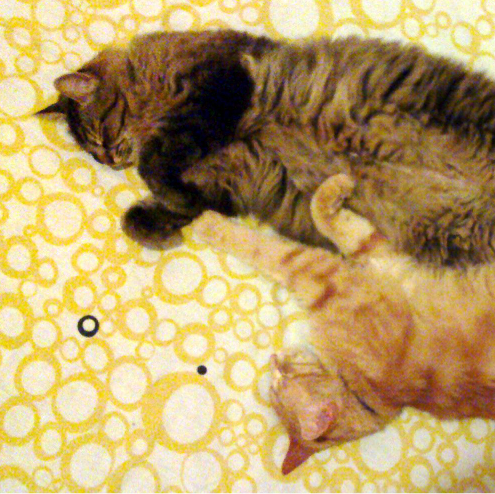
\includegraphics[width=\marginparwidth]{cats}
    \caption{In this image, the cats are tessellated within a square
      frame. Images should also have captions and be within the
      boundaries of the sidebar on page~\pageref{bar:sidebar}. Photo:
      \cczero~jofish on Flickr.}
    \label{fig:marginfig}
\end{marginfigure}

\section{Figures}
The examples on this and following pages should help you get a feel
for how screen-shots and other figures should be placed in the
template. Your document may use color figures (see
Figures~\ref{fig:sample}), which are included in the page limit; the
figures must be usable when printed in black and white. You can use
the \texttt{marginfigure} environment to insert figures in the (left) margin
of the document (see Figure~\ref{fig:marginfig}). Finally, be sure to
make images large enough so the important details are legible and
clear (see Figure~\ref{fig:cats}).

\begin{figure*}
  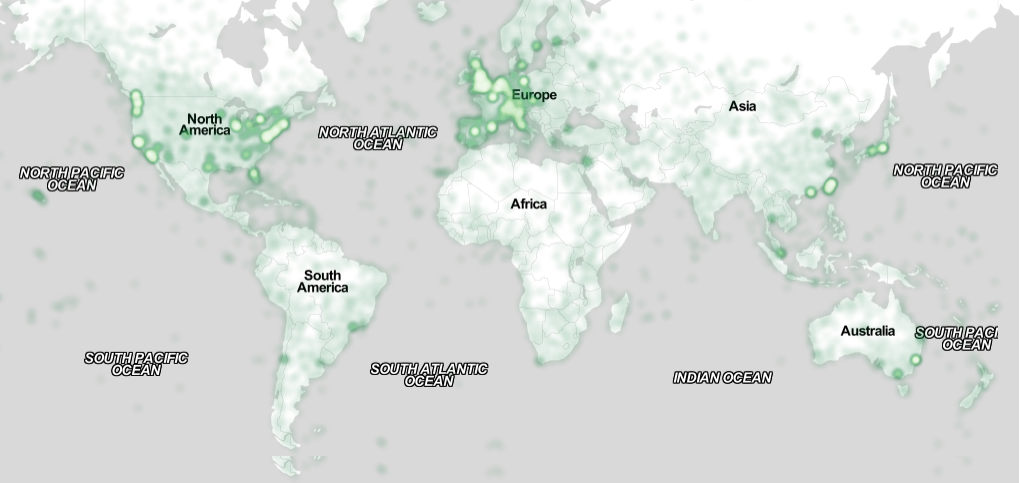
\includegraphics[width=\fulltextwidth]{map}
  \caption{In this image, the map maximizes use of space.
    Note that \LaTeX\ tends to render large figures on a
    dedicated page. Image: \ccbynd~ayman on Flickr.}~\label{fig:cats}
\end{figure*}


\section{Tables}


\begin{margintable}
    \caption{A simple narrow table in the left margin
      space.}
    \label{tab:table2}
    \begin{tabular}{r r l}
      & {\small \textbf{First}}
      & {\small \textbf{Location}} \\
      \toprule
      Child & 22.5 & Melbourne \\
      Adult & 22.0 & Bogot\'a \\
      \midrule
      Gene & 22.0 & Palo Alto \\
      John & 34.5 & Minneapolis \\
      \bottomrule
    \end{tabular}
\end{margintable}

You man use tables inline with the text (see Table~\ref{tab:table1})
or within the margin as shown in Table~\ref{tab:table2}. Try to
minimize the use of lines (especially vertical lines). \LaTeX\ will
set the table font and captions sizes correctly; the latter must
remain unchanged.

\section{Accessibility}
The Executive Council of SIGCHI has committed to making SIGCHI
conferences more inclusive for researchers, practitioners, and
educators with disabilities. As a part of this goal, the all authors
are asked to work on improving the accessibility of their
submissions. Specifically, we encourage authors to carry out the
following five steps:
\begin{itemize}
\item Add alternative text to all figures
\item Mark table headings
\item Generate a tagged PDF
\item Verify the default language
\item Set the tab order to ``Use Document Structure''
\end{itemize}

For links to instructions and resources, please see:
\url{http://chi2016.acm.org/accessibility}

Unfortunately good tools do not yet exist to create tagged PDF files
from Latex (see the ongoing effort at
\url{http://tug.org/twg/accessibility/}). \LaTeX\ users will need to
carry out all of the above steps in the PDF directly using Adobe
Acrobat, after the PDF has been generated.

For more information and links to instructions and resources, please
see:
\url{http://chi2016.acm.org/accessibility} and
\url{http://tug.org/twg/accessibility/}.  


\section{Producing and Testing PDF Files}

We recommend that you produce a PDF version of your submission well
before the final deadline. Your PDF file must be ACM DL Compliant and
meet stated requirements,
\url{http://www.sheridanprinting.com/sigchi/ACM-SIG-distilling-settings.htm}.

\begin{sidebar}
  So long as you don't type outside the right
  margin or bleed into the gutter, it's okay to put annotations over
  here on the left. You may need to have
  to manually align the margin paragraphs to your \LaTeX\ floats using
  the \texttt{{\textbackslash}vspace{}} command.
\end{sidebar}


Test your PDF file by viewing or printing it with the same software we
will use when we receive it, Adobe Acrobat Reader Version 10. This is
widely available at no cost. Note that most reviewers will use a North
American/European version of Acrobat reader, so please check your PDF
accordingly.

\begin{acks}
  We thank all the volunteers, publications support, staff, and
  authors who wrote and provided helpful comments on previous versions
  of this document. As well authors 1, 2, and 3 gratefully acknowledge
  the grant from \grantsponsor{001}{NSF}{}
  (\#\grantnum{001}{1234-2222-ABC}). Author 4 for example may want to
  acknowledge a supervisor/manager from their original employer. This
  whole paragraph is just for example. Some of the references cited in
  this paper are included for illustrative purposes only.
\end{acks}

\section{References Format}

Your references should be published materials accessible to the
public. Internal technical reports may be cited only if they are
easily accessible and may be obtained by any reader for a nominal fee.
Proprietary information may not be cited. Private communications
should be acknowledged in the main text, not referenced (e.g.,
[Golovchinsky, personal communication]). References must be the same
font size as other body text. References should be in alphabetical
order by last name of first author. Use a numbered list of references
at the end of the article, ordered alphabetically by last name of
first author, and referenced by numbers in brackets. For papers from
conference proceedings, include the title of the paper and the name of
the conference. Do not include the location of the conference or the
exact date; do include the page numbers if available.

References should be in ACM citation format:
\url{http://www.acm.org/publications/submissions/latex_style}.  This
includes citations to Internet
resources~\cite{CHINOSAUR:venue,cavender:writing,psy:gangnam}
according to ACM format, although it is often appropriate to include
URLs directly in the text, as above. Example reference formatting for
individual journal articles~\cite{ethics}, articles in conference
proceedings~\cite{Klemmer:2002:WSC:503376.503378},
books~\cite{Schwartz:1995:GBF}, theses~\cite{sutherland:sketchpad},
book chapters~\cite{winner:politics}, an entire journal
issue~\cite{kaye:puc},
websites~\cite{acm_categories,cavender:writing},
tweets~\cite{CHINOSAUR:venue}, patents~\cite{heilig:sensorama}, 
games~\cite{supermetroid:snes}, and
online videos~\cite{psy:gangnam} is given here.  See the examples of
citations at the end of this document and in the accompanying
\texttt{BibTeX} document. This formatting is a edited version of the
format automatically generated by the ACM Digital Library
(\url{http://dl.acm.org}) as ``ACM Ref''. DOI and/or URL links are
optional but encouraged as are full first names. Note that the
Hyperlink style used throughout this document uses blue links;
however, URLs in the references section may optionally appear in
black.





\bibliography{sigchi-a}
\bibliographystyle{ACM-Reference-Format}

\end{document}
